\section{Motivational Example}
\label{sec:motiv}
% an examples to illustrate what do we mean by automation and what are different data sources changes taking dependencies into account. 
% Speaking of challenges in building such a system such as
To better understand the ECiDA project's motivations, we present an example from various real-world data analysis applications. Further will use this example through this document to explain each section. 

The ever increasing development in data science enables industries to use data-centric projects ranging from healthcare \cite{qadri2020future} to manufacturing \cite{ismail2019manufacturing}. Predictive maintenance is one of these projects for preventing failure in productions, especially in Industry 4.0. Different applications are defined in this field, such as predicting the remaining useful life of a machine using data analysis techniques can avoid damage to the industry by replacing the device at the right time also to minimize the operating expenses \cite{mobley2002introduction}. 

Figure \ref{fig:example} shows an overview of a sample predictive maintenance pipeline derived from literature in related field \cite{sahal2020big,yamato2016proposal,short2019industrial}. This pipeline collects streaming data from sensors and analyzes data to extract useful insights for maintenance use cases. Besides, a batch processing pipeline receives all data points and evaluates the streaming pipeline's performance instead of analyzing only the events. Using feedbacks from batch processing, we should update the stream processing pipeline to improve the accuracy, e.g. by capturing new events. It is critical to have the streaming pipeline up and running 24x7 and to deliver the updates as soon as possible to prevent irrecoverable damages. For example, a malfunction in a boiler or toxic water could put lives in danger, while a timely update in the stream processing pipeline could prevent the catastrophe. 

The more data and the more variant data types improve the predictive model's potential to reach better performance. Various sources are used for predictive maintenance, visual inspections such as thermal imaging, physical conditions such as noise generated by the device, internal device states. Some may want to start with visual inspection first and then add other sensors to make the model more accurate over time. In fig. \ref{fig:example}, the input sources are represented as hexagons. Each sensor is placed on several devices. For example, the thermometers are installed on boilers, motors, and pumps. 

Event detection components are on the next layer. They collect data from sensors and find pre-defined patterns in data to capture unique events. Extracting useful information in the first layer reduces network usage and response time. For instance, a thermometer is installed on a motor, and the heat detector captures events when the temperature is above a threshold. Another instance is an event detector looking for an event when the device is rattling and loud to anticipate motor malfunction. Since there are different devices, we may need to have distinct event detectors for each device types, e.g. the threshold differentiates between a motor and pump.

Next, the aggregator collects data points from different (in type and device) sources and order them chronologically, then joins them by device and timestamp such that each record represents every event that occurred at a specific time on a particular machine. In this component, input data points are dependent as they formed an output record together. 

The desired applications are placed in the next layer, where all components receive data from the aggregator. Each component works independently and analyzes data to produce the desired outcome. For instance, the failure prediction can predict an upcoming malfunction happening shortly if the motor temperature unexpectedly goes high while it is rattling and generating intense noise. 

Whenever a result is ready, the applications will send it to the end-point that is responsible for acting on the insights. If there is a critical issue in the company, instantly act upon that, like shutting down the motor. Otherwise, alarm the operator. Although this component receives three distinct inputs, the inputs are independent, and actions are defined per input. 

\begin{figure}[ht]
    \centering
    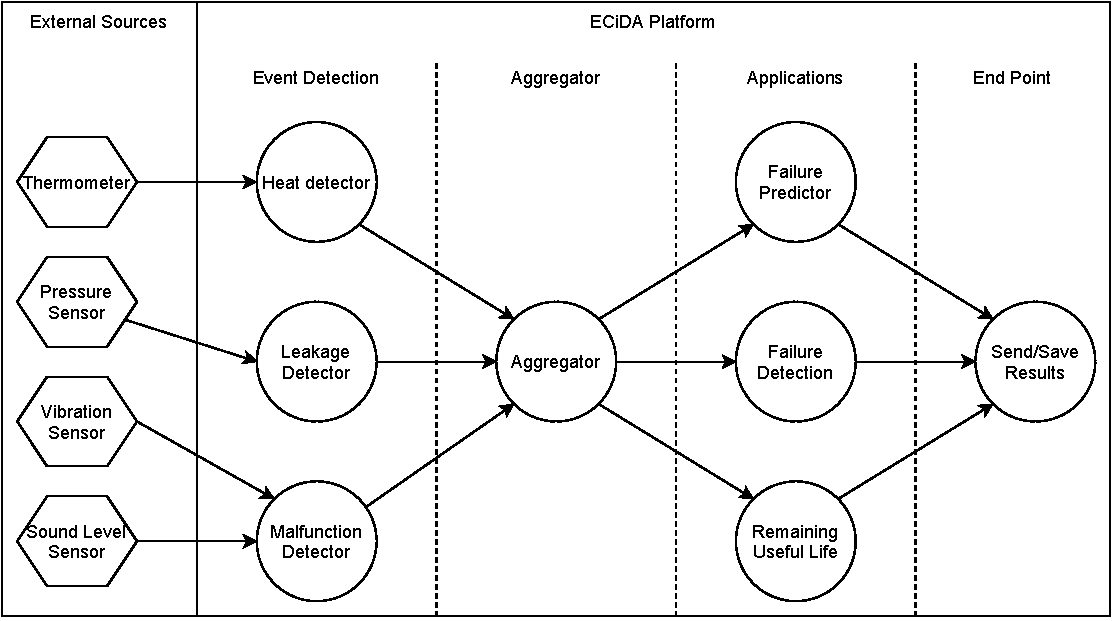
\includegraphics[width=1\textwidth]{example/example.pdf}
    \caption{\textbf{A predictive maintenance pipeline:} Circles are controllable components inside the ECiDA platform, while the hexagons are external sensors.}
    \label{fig:example}
\end{figure}

As mentioned above, a batch processing application runs periodically to analyze the whole data (not just events) and also evaluate the streaming pipeline performance. We can update the real-time pipeline according to the insights from the entire data point set and the actual events that happened in the real world, which can assess the predictions. A resulting update can happen in any component.

We may want to update the currently running model in the application layer to a newly trained model. We may also want to capture new events by adding more event detectors leading to updating the aggregator. We may even find that an event is of no use in the prediction and only occupied resources, and it is better to be removed from the pipeline. The change might be subtle such as changing the threshold, or it could be as immense as changing the entire pipeline, including components and connections. 
